\section{Introducció}
{
    En els darrers anys, els serveis de contingut en temps real han experimentat un creixement quasi exponencial, sobretot arran de la
    popularitat de pàgines web com \url{youtube.com}, \url{twitch.tv} o sobretot amb l'ús de les videoconferències durant la pandèmia.
    No obstant això, les tècniques actuals per distribuir aquest tipus de contingut, malgrat haver millorat bastant amb el desenvolupament
    d'eines com \ac{WebRTC}, encara representen un problema molt greu tant a la part dels servidors, principalment per les \ac{CDN}, com també pel
    volum de tràfic que implica a les xarxes, principalment pels \ac{ISP}. De fet, s'està tornant una qüestió tecnològica tant greu que molts
    serveis d'aquests han decidit apujar els seus preus per poder fer front a la demanda.
    \footnote{\href{https://www.xataka.com/empresas-y-economia/13-grandes-operadoras-se-unen-para-volver-a-pedir-a-europa-pago-tuberias-que-servicios-como-netflix-youtube-ayuden-costes-red}{Notícia a Xataka el 29-11-21: 13 operadoras piden subir precios a Netflix y Youtube.}}

    Al mateix temps que hi ha aquest augment de la demanda per serveis nous d'Internet, també hi ha altres que estan intentant canviar
    de plataforma de distribució tecnològica com la televisió i la ràdio; és a dir, les cadenes de televisió estan intentant transmetre el seu contingut utilitzant Internet en lloc d'antenes i cable. 
    De fet, fer-ho a través d'Internet permet estalviar costos significatius de distribució al mateix temps que permet tenir una retroactivitat i perspectiva més acurada
    de la quantitat de gent que està veient l'emissió.

    \begin{figure}[H]
        \label{fig:trafic_desglosat}
        \centering
        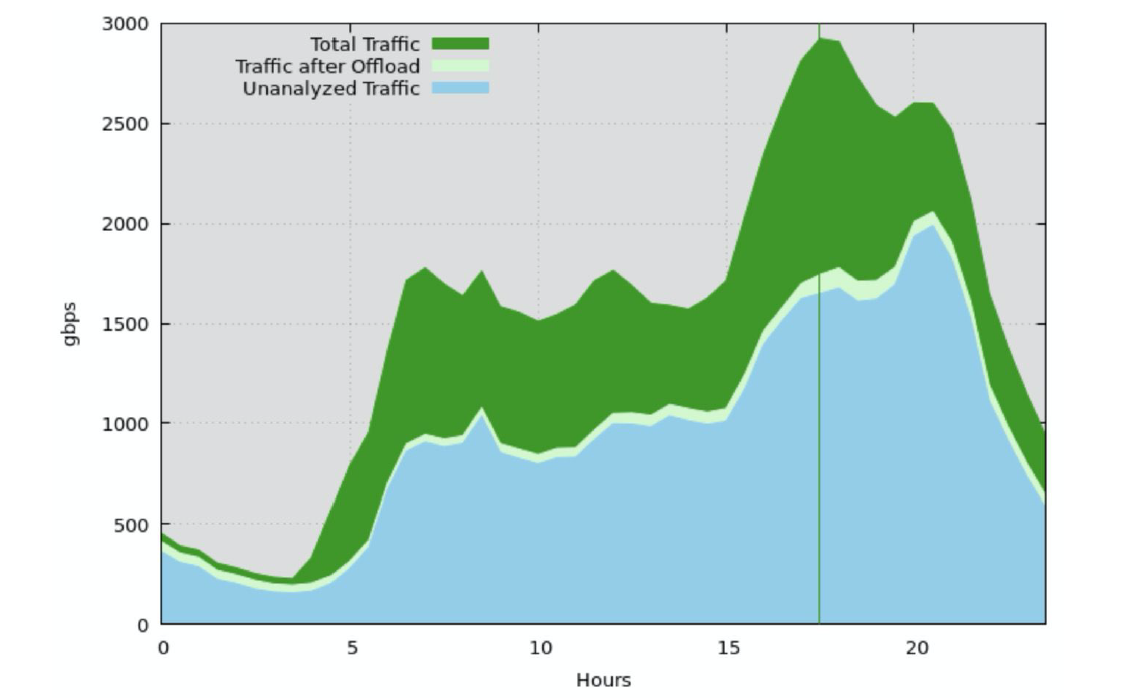
\includegraphics[width=15cm, height=7.2cm]{img/01_introduccio/trafic_peak.png}
        \caption[Trafic d'Internet]{\footnotesize{Volum de tràfic en un dia amb la sortida d'un nou videojoc. En blau el tràfic no analitzat,
        en ver fort el tràfic normal, en verd fluix el tràfic si la descarrega es fes amb multicast. Imatge d'Akamai.}}
    \end{figure}

    L'any 2015, el tràfic de serveis de vídeo en temps real, com Netflix, YouTube o Twitch, va representar pràcticament el 70\% del tràfic.
    \footnote{\href{https://hipertextual.com/2015/12/streaming-netflix-ancho-banda}{Notícia a Hipertextual el 07-12-15: El streaming ya representa el 70\% del tráfico de la red}}
    Normalment, aquest tipus de tràfic va per pics, ja que quan una nova temporada d'una sèrie famosa, quan un youtuber important puja un nou vídeo o s'està
    fent un esdeveniment en directe la quantitat de gent veient el contingut sol augmentar de manera sobtada sobretot als primers moments. Això sol implicar
    en general problemes per donar accés a tothom al servei depenent de quanta gent sigui, mentre que al mateix temps altres serveis també es vegin
    afectats (les \ac{CDN} solen tenir molts serveis simultàniament distribuïts en microserveis).
    
    \newpage

    Per ficar dades i posar-nos en context del volum de tràfic, el màxim que s'ha arribat a donar simultàniament per part de la \ac{CDN} Akamai
    ha estat un pico de 200 Tbps en març de 2021.\footnote{\href{https://addvalue.com.br/novo/artigos/akamai-hits-huge-new-200-tbps/}{Noticia a Addvalue el 24-03-22: Akamai hits huge new 200 Tbps web traffic peak}}
    Suposant un tràfic lineal, per simplificar, ja que normalment s'utilitzen codificacions \ac{CBR}
    en directe en temps real, amb una resolució de 1080p el tràfic és de 5 Mbps/connexió i fins a 20 Mbps/connexió en cas de 4k. Llavors, en 1080p
    suposant aquell tràfic màxim suportat llavors es podrien arribar fins a 40 milions de clients en 1080p i fins a 10 milions en 4k. Si tota
    Espanya volgués mirar un contingut en directe, seria quasi impossible donar el servei correctament en 4k i molt just en 1080p.
    
    Aquests problemes de subministrament solen ser a causa de que les connexions que es fan són punt a punt; dit d'una altra manera,
    són \textbf{unicast}. Això implica que el servei que pots donar en gran part està limitat al nombre de connexions simultànies que es pot suportar. Malgrat que
    l'ús d'unicast té grans avantatges com la facilitat en la seguretat, la simplificació en l'arquitectura del programa o que pràcticament tots els
    dispositius del món ho suporten de manera nativa, també comporta un gran inconvenient.
    
    Si el contingut que has de distribuir als clients és exactament el mateix com en el cas de la televisió o la ràdio, unicast pot arribar a saturar
    un servei si el volum d'usuaris és molt alt. Amb això en ment, ja a finals dels anys 80 es va publicar una extensió de d'\ac{IP}, \cite{RFC 988} que solucionava
    aquest problema: \textbf{IP Multicast}. Malgrat no estar tan establerta com IP unicast, sí que la gran majoria de dispositius l'accepten.
    
    Per altra banda, al llarg dels anys, a les connexions unicast normalment han fet ús d'un protocol anomenat \ac{TCP}. Aquest protocol va ser especialment
    important en els anys 90 i a principis dels 2000 perquè Internet pogués funcionar i popularitzar-se, ja que les connexions eren lentes i poc fiables.
    Aquest protocol incorpora una sèrie de mecanismes per intentar pal·liar aquesta qüestió. No obstant això, amb la millora de les connexions i la seva fiabilitat
    hi ha altres protocols que poden ser més útils i millors en l'Internet que tenim actualment, incorporant funcionalitats que antigament no s'havien plantejat
    o que no semblaven rellevants. Un protocol que pareix que substituirà \ac{TCP} és QUIC, ja que millora bastant certs aspectes de TCP com l'establiment
    de la connexió molt més ràpidament (menys RTTs) o el fet de poder restablir la sessió amb el servidor en canviar de xarxa.
    
}

\subsection{Transfons del project}
{
    Aquest projecte es fa des de cero, encara agafa principalment dos projectes de codi lliure d'Internet i un borrador del \ac{IETF}:

    \begin{enumerate}
        \item{\textbf{\textit{Hypertext Transfer Protocol (\ac{HTTP}) over multicast QUIC}}, de Lucas Pardue, Richard Bradbury i Sam Hurst.}
        \item{\textbf{\textit{NGHQ}}: Llibrería escrita en C que implementa part de l'esborrany de \textit{\ac{HTTP} sobre multicast QUIC} fins la versió 7.}
        \item{\textbf{\textit{NGTCP2}}: Llibrería escrita en C que implementa el protocol QUIC segons l'estàndard escrit en el \ac{RFC} 9000.}
    \end{enumerate}

    La idea original ha estat de l'autor, encara que l'enfocament i la metodologia han estat proposades pel professor, Jorge Mata.

    Tot el codi utilitzat és de codi lliure desenvolupat per enginyers i que està pràcticament tot allotjat en plataformes
    online com Github. Tot el codi desenvolupat en aquest projecte està allotjat també al Github i també és de codi lliure.
}

\subsection{Objectius}
{
    \begin{itemize}
        \item Desenvolupar un servidor servidor QUIC unicast i un servidor QUIC multicast per distribuir contingut en temps real.
        \item Conèixer en profunditat les avantatges i limitacions de la tecnologia QUIC \cite{rfc9000}
        \item Discutir la possibilitat de fer un perfil concret de QUIC per Multicast.
        \item Demostrar les limitacions d'unicast en la retransmissions a un gran número de clients i com Multicast pot ser una solució.
    \end{itemize}
}

\subsection{Requeriments i especificacions}
{
    \textbf{Requeriments del projecte}:
    \begin{itemize}
        \item Proveir un sistema de transmissió de contingut en directe via unicast i/o multicast.
        \item Possibilitat l'avaluació del tràfic generat de manera quantitativa i qualitativa.
        \item Implementar software gratuït i de codi lliure.
        \item Proveir una guia a l'usuari final per facilitar l'ús i instal·lació dels softwares tant
                del client com del servidor [Annexe I].
    \end{itemize}
    
    \textbf{Especificacions del projecte}:
    \begin{itemize}
        \item Avaluar el tràfic generat per multicast i unicast en escenaris amb diversos clients escoltant
                la retransmissió.
        \item Creació d'un entorn de proves virtual, on el servidor i els clients seràn màquines virtuals Linux.
        \item Avaluar el tràfic amb eines d'ús extensiu, proveint els filtres necessaris per descodificar els missatges transmesos.
    \end{itemize}
}

\subsection{Pla de feina}
{
    En aquesta secció de document es descriu en detall tots els blocs de treball en el qual s'ha dividit la feina i els temps (Diagrama de Gantt)
    en els que s'ha fet la tasca corresponent.
    
    Al llarg del projecte, hi ha hagut diversos canvis en respecte al pla original. Els principals canvis han estat els següents:
    \begin{itemize}
        \item \textbf{Lectura de \ac{RFC}s}. Donat la complexitat del projecte i la profunditat d'aquest s'ha vist que la quantitat de documentació
        al respecte que s'ha hagut de llegir ha estat molt major de la qual s'esperava, en gran part, ja que el nombre de tecnologies
        necessaries per poder entendre i desenvolupar una plataforma com la que es demana és molt major del qual es podria esperar a priori.
        També, a causa que s'utilitzen tecnologies noves com QUIC, hi ha hagut \ac{RFC}s que han aparegut durant el transcurs com el 9221.
        \item \textbf{Certs programes no existien o no compilaven}. Per fer l'escenari de proves s'ha volgut fer servir un software nou per virtualitzar
        la xarxa intentant imitar la de la pràctica \ac{IP} multicast de l'assignatura \ac{TCGI} del grau d'Enginyeria de serveis i sistemes
        de telecomunicaciones del \ac{ETSETB}. Es va trobar que les màquines virtuals i el software utilitzat en aquelles màquines és antic i qualcun
        ja no està disponible. S'ha buscat alternatives al respecte.
        
        El que més ha dificultat i endarrerit el desenvolupament ha estat la lectura de la documentació, ja que era molt més extensa del que s'esperava a priori
        a més que també entrava en molts detalls que semblaven contradictoris amb la idea, encara que sembla que no. S'ha de pensar que la proposta és una
        tecnologia que encara no s'ha desenvolupat del tot i encara està en procés, llavors això és més una prova del concepte que una demostració per ficar-ho
        a producció. Encara s'està lluny d'aquest punt com es veurà al llarg del treball.
    \end{itemize}
}
\subsubsection{Estructura de la feina}
{
    \textbf{[ESBORRANY - FALTA L'IMATGE FINAL]}
    \begin{figure}[H]
        \label{fig:estructura}
        \centering
        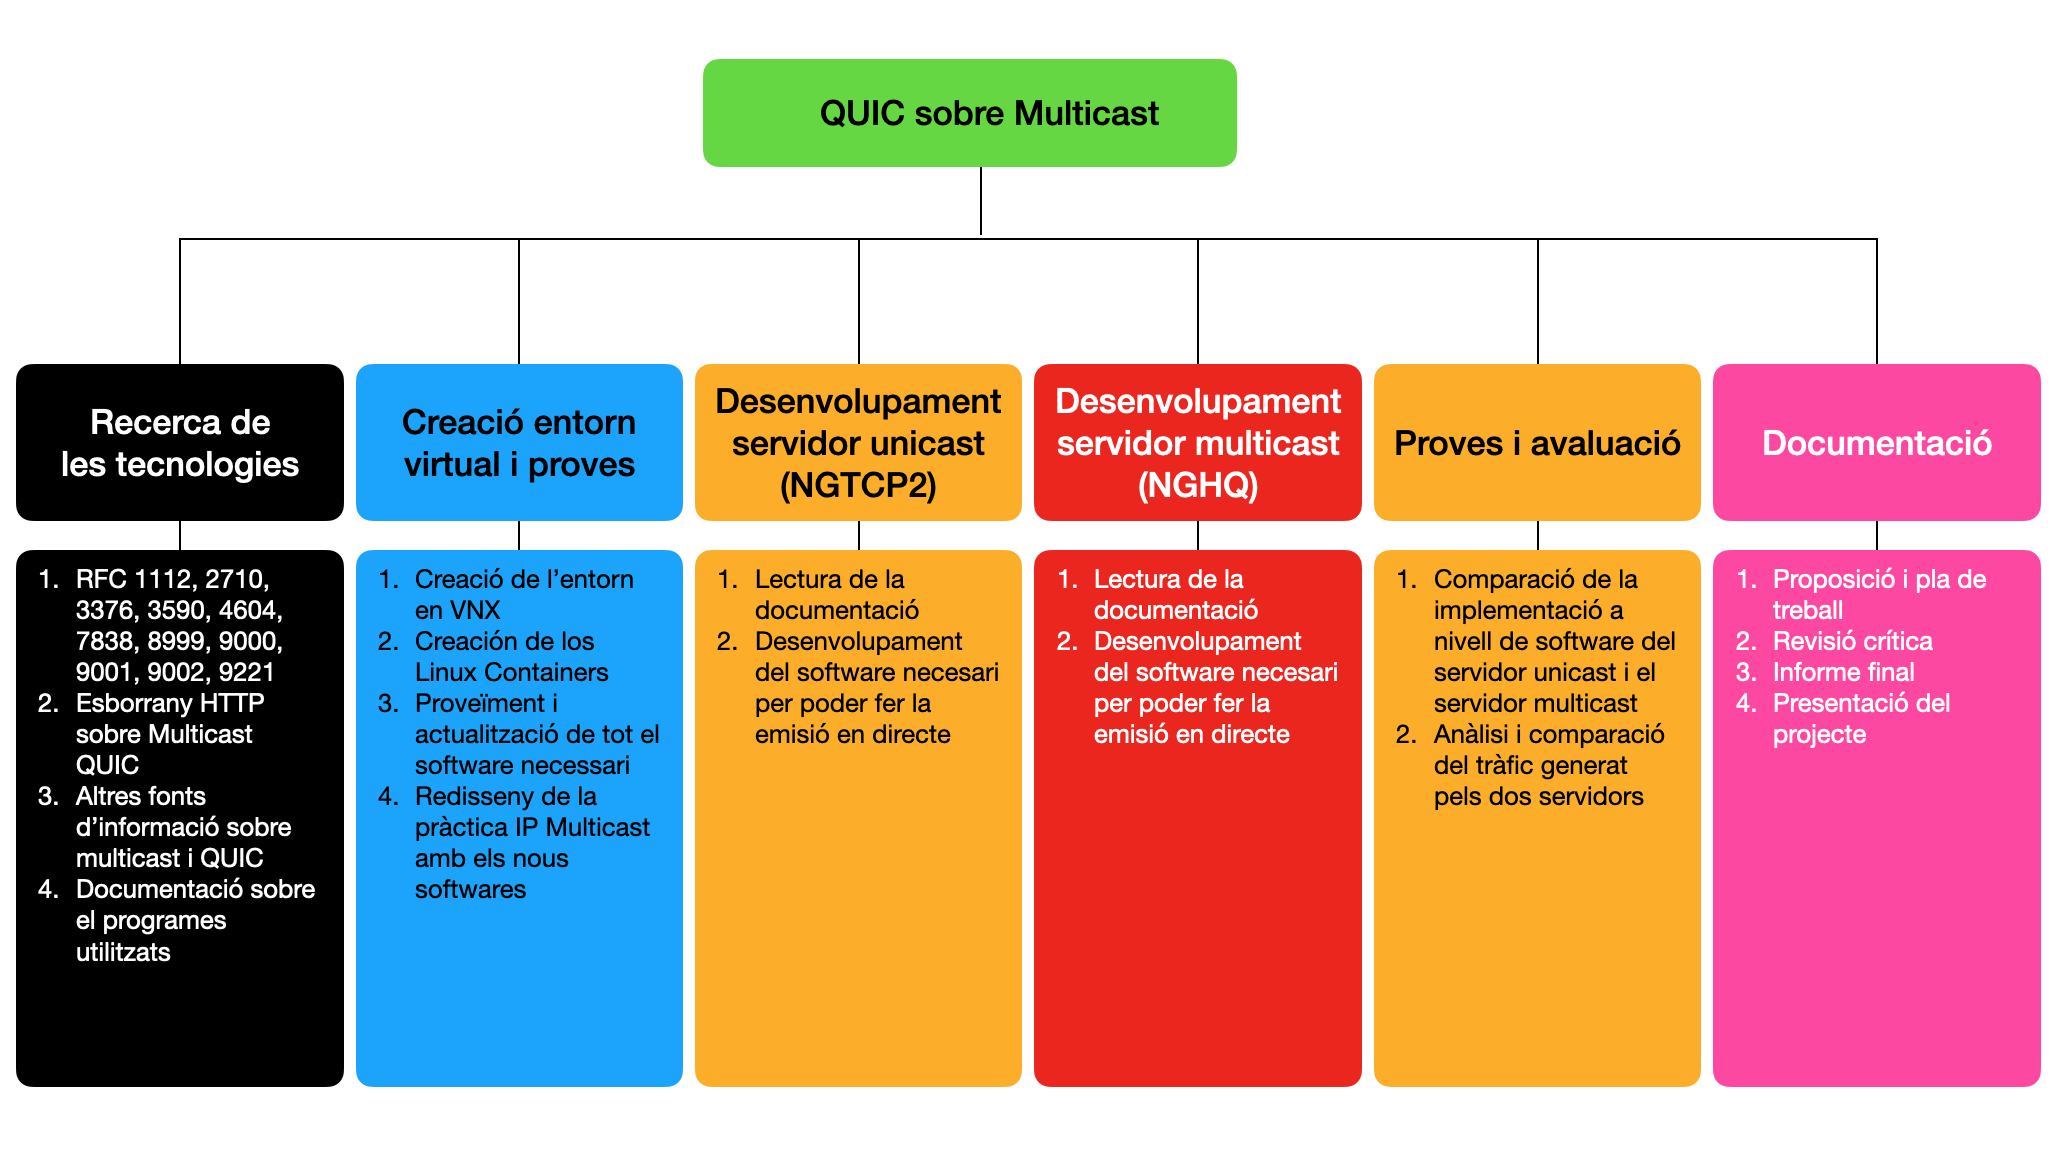
\includegraphics[width=15cm]{img/01_introduccio/estructura_treball.png}
    \end{figure}
}
\subsubsection{Paquets de feina, tasques i fites}
{
    \begin{center}
        
\begin{table}[H]
    \begin{tabular}{|l|ll|l}
    \cline{1-3}
    Projecte: \textbf{Recerca de les tecnologies}                                                                                                                                                                                                                                          & \multicolumn{2}{l|}{WP ref: \textbf{WP1}}                                                                                                                                               &  \\ \cline{1-3}
    Element principal: Lectura de la documentació                                                                                                                                                                                                                                                      & \multicolumn{2}{l|}{Pàg. 1 de 6}                                                                                                                                               &  \\ \cline{1-3}
    \multirow{2}{*}{\begin{tabular}[c]{@{}l@{}}Breu descripció: \\ Lectura del RFCs necessaris per tal d'entendre i proposar\\ solucions adequades per crear un perfil de QUIC sobre\\ multicast.\\ \\ Lectura de la documentació necesaria\end{tabular}}                                            & \multicolumn{2}{l|}{\begin{tabular}[c]{@{}l@{}}Data d'inici estimada:\\              01-10-2021 \\ Data de finalització estimada: \\                01-11-2021\end{tabular}} &  \\ \cline{2-3}
                                                                                                                                                                                                                                                                                                       & \multicolumn{2}{l|}{\begin{tabular}[c]{@{}l@{}}Data d'inici real:\\                14-09-2021 \\ Data de finalització real:\\           30-04-2022\end{tabular}}        &  \\ \cline{1-3}
    \begin{tabular}[c]{@{}l@{}}Tasques internes:\\ \\ T1. RFC 1112, 2710, 3376, 3590, 4604, 7838, 8999,\\        9000, 9001, 9002, 9221\\ T2. Esborrany HTTP sobre Multicast QUIC\\ T3. Altres fonts d'informació sobre multicast i QUIC\\ T4. Documentació sobre el programes utilitzats\end{tabular} & \multicolumn{1}{l|}{\begin{tabular}[c]{@{}l@{}}Entregables:\\ Tasca 1 i 2\end{tabular}}    & \begin{tabular}[c]{@{}l@{}}Dates:\\ incluides\\ en el\\ document\end{tabular}    &  \\ \cline{1-3}
    \end{tabular}
    \end{table}
        \begin{table}[H]
    \begin{tabular}{|l|ll|l}
    \cline{1-3}
    Projecte: \textbf{Creació entorn virtual i proves}                                                                                                                                                                                                                                          & \multicolumn{2}{l|}{WP ref: \textbf{WP2}}                                                                                                                                                                   &  \\ \cline{1-3}
    Element principal: Entorn virtual                                                                                                                                                                                                                                              & \multicolumn{2}{l|}{Pàg. 2 de 6}                                                                                                                                                                   &  \\ \cline{1-3}
    \multirow{2}{*}{\begin{tabular}[c]{@{}l@{}}Breu descripció: \\ Creació de l'entorn virtual amb VNX, proveïment \\ de les màquines virtuals amb el software necesari i\\ fer la pràctica d'IP multicast de TCGI per testejar\\ que l'entorn funciona correctament\end{tabular}}   & \multicolumn{2}{l|}{\begin{tabular}[c]{@{}l@{}}Data d'inici estimada:\\               16-09-2021\\  Data de finalització estimada:\\                10-10-2021\end{tabular}}                     &  \\ \cline{2-3}
                                                                                                                                                                                                                                                                                       & \multicolumn{2}{l|}{\begin{tabular}[c]{@{}l@{}}Data d'inici real:\\                16-09-2021\\ Data de finalització real:\\                30-12-2022\end{tabular}}                            &  \\ \cline{1-3}
    \begin{tabular}[c]{@{}l@{}}Tasques internes:\\ \\ T1. Creació de l'entorn en VNX\\ T2. Creació dels Linux Containers\\ T3. Proveïment i actualització de tot el software\\       necessari\\ T4. Rediseny de la pràctica IP Multicast amb \\       els nous softwares\end{tabular} & \multicolumn{1}{l|}{\begin{tabular}[c]{@{}l@{}}Entregables:\\ Presentació al\\ professor de \\ l'escenari\\ montat\end{tabular}} & \begin{tabular}[c]{@{}l@{}}Dates:\\ 14-01-2022\\ \end{tabular} &  \\ \cline{1-3}
    \end{tabular}
    \end{table}
        \begin{table}[H]
    \begin{tabular}{|l|ll|l}
    \cline{1-3}
    \begin{tabular}[c]{@{}l@{}}Projecte: \textbf{Desenvolupament servidor} \\                \textbf{unicast (NGTCP2)}\end{tabular}                                                                                                                                  & \multicolumn{2}{l|}{WP ref: \textbf{WP3}}                                                                                                                                            &  \\ \cline{1-3}
    Element principal: Desenvolupament de software                                                                                                                                                                                                 & \multicolumn{2}{l|}{Pàg. 3 de 6}                                                                                                                                            &  \\ \cline{1-3}
    \multirow{2}{*}{\begin{tabular}[c]{@{}l@{}}Breu descripció:\\ \\ Creació d'un servidor unicast que utilitzi el protocol\\ QUIC per poder utilitzar-lo per comparar amb un\\ que utilitzi multicast. També s'ha de fer el client.\end{tabular}} & \multicolumn{2}{l|}{\begin{tabular}[c]{@{}l@{}}Data d'inici estimada:\\               01-11-2021\\ Data de finalització estimada:\\                01-12-2021\end{tabular}} &  \\ \cline{2-3}
                                                                                                                                                                                                                                                   & \multicolumn{2}{l|}{\begin{tabular}[c]{@{}l@{}}Data d'inici real:\\                15-02-2022\\ Data de finalització real:\\                05-05-2022\end{tabular}}        &  \\ \cline{1-3}
    \begin{tabular}[c]{@{}l@{}}Tasques internes:\\ \\ T1. Lectura de la documentació\\ T2. Desenvolupament del software necesari per poder\\        per poder fer la emisió en directe.\end{tabular}                                               & \multicolumn{1}{l|}{\begin{tabular}[c]{@{}l@{}}Entregables:\\ Tasca 1\\ Tasca 2\\ Tasca 3\end{tabular}}   & \begin{tabular}[c]{@{}l@{}}Dates:\\ 15-05-2022\end{tabular}   &  \\ \cline{1-3}
    \end{tabular}
    \end{table}
        \begin{table}[H]
    \begin{tabular}{|l|ll|l}
    \cline{1-3}
    \begin{tabular}[c]{@{}l@{}}Projecte: \textbf{Desenvolupament servidor} \\                \textbf{multicast (NGHQ)}\end{tabular}                                                                                                                                  & \multicolumn{2}{l|}{WP ref: \textbf{WP4}}                                                                                                                                            &  \\ \cline{1-3}
    Element principal: Desenvolupament de software                                                                                                                                                                                                 & \multicolumn{2}{l|}{Pàg. 4 de 6}                                                                                                                                            &  \\ \cline{1-3}
    \multirow{2}{*}{\begin{tabular}[c]{@{}l@{}}Breu descripció:\\ \\ Creació d'un servidor multicast que utilitzi el protocol\\ QUIC per poder utilitzar-lo per comparar amb un\\ que utilitzi unicast. També s'ha de fer el client.\end{tabular}} & \multicolumn{2}{l|}{\begin{tabular}[c]{@{}l@{}}Data d'inici estimada:\\               01-11-2021\\ Data de finalització estimada:\\                01-12-2021\end{tabular}} &  \\ \cline{2-3}
                                                                                                                                                                                                                                                   & \multicolumn{2}{l|}{\begin{tabular}[c]{@{}l@{}}Data d'inici real:\\                15-02-2022\\ Data de finalització real:\\                05-05-2022\end{tabular}}        &  \\ \cline{1-3}
    \begin{tabular}[c]{@{}l@{}}Tasques internes:\\ \\ T1. Lectura de la documentació\\ T2. Desenvolupament del software necesari per poder\\        per poder fer la emisió en directe.\end{tabular}                                               & \multicolumn{1}{l|}{\begin{tabular}[c]{@{}l@{}}Entregables:\\ Tasca 1\\ Tasca 2\\ Tasca 3\end{tabular}}   & \begin{tabular}[c]{@{}l@{}}Dates:\\ 15-05-2022\end{tabular}   &  \\ \cline{1-3}
    \end{tabular}
    \end{table}
        % Please add the following required packages to your document preamble:
% \usepackage{multirow}
\begin{table}[H]
    \begin{tabular}{|l|ll|l}
    \cline{1-3}
    Projecte: \textbf{Proves i avaluació}                                                                                                                                                                                                              & \multicolumn{2}{l|}{WP ref: \textbf{WP5}}                                                                                                                                            &  \\ \cline{1-3}
    Element principal: Simulació i proves de qualitat                                                                                                                                                                                         & \multicolumn{2}{l|}{Pàg. 5 de 6}                                                                                                                                            &  \\ \cline{1-3}
    \multirow{2}{*}{\begin{tabular}[c]{@{}l@{}}Breu descripció:\\ \\ Totes les simulacions i  avaluacions necessaries\\ per aconseguir proves concloents de en quin cas\\ és millor utilitzar unicast i quin multicast.\end{tabular}}         & \multicolumn{2}{l|}{\begin{tabular}[c]{@{}l@{}}Data d'inici estimada:\\               01-11-2021\\ Data de finalització estimada:\\                15-12-2021\end{tabular}} &  \\ \cline{2-3}
                                                                                                                                                                                                                                              & \multicolumn{2}{l|}{\begin{tabular}[c]{@{}l@{}}Data d'inici real:\\                15-02-2022\\ Data de finalització real:\\                05-05-2022\end{tabular}}        &  \\ \cline{1-3}
    \begin{tabular}[c]{@{}l@{}}Tasques internes:\\ \\ T1. Comparació de l'implementació a nivell de\\ software del servidor unicast i el servidor\\ multicast\\ T2. Anàlisi i comparació del tràfic generat pels\\ dos servidors\end{tabular} & \multicolumn{1}{l|}{\begin{tabular}[c]{@{}l@{}}Entregables:\\ Tasca 1\\ Tasca 2\\ Tasca 3\end{tabular}}   & \begin{tabular}[c]{@{}l@{}}Dates:\\ 15-05-2022\end{tabular}   &  \\ \cline{1-3}
    \end{tabular}
    \end{table}
        % Please add the following required packages to your document preamble:
% \usepackage{multirow}
\begin{table}[H]
    \begin{tabular}{|l|ll|l}
    \cline{1-3}
    Projecte: \textbf{Documentació}                                                                                                                                                                                          & \multicolumn{2}{l|}{WP ref: \textbf{WP6}}                                                                                                                                                                     &  \\ \cline{1-3}
    Element principal: Documentació                                                                                                                                                                                 & \multicolumn{2}{l|}{Pàg. 6 de 6}                                                                                                                                                                     &  \\ \cline{1-3}
    \multirow{2}{*}{\begin{tabular}[c]{@{}l@{}}Breu descripció:\\ \\ Documentació que s'ha d'entregar. Un manual\\ d'usuari per poder configurar ambdos servidors\\ serà inclós en el document final.\end{tabular}} & \multicolumn{2}{l|}{\begin{tabular}[c]{@{}l@{}}Data d'inici estimada:\\               15-09-2021\\ Data de finalització estimada:\\                15-01-2022\end{tabular}}                          &  \\ \cline{2-3}
                                                                                                                                                                                                                    & \multicolumn{2}{l|}{\begin{tabular}[c]{@{}l@{}}Data d'inici real:\\                20-01-2022\\ Data de finalització real:\\                15-05-2022\end{tabular}}                                 &  \\ \cline{1-3}
    \begin{tabular}[c]{@{}l@{}}Tasques internes:\\ \\ T1. Proposició i pla de treball\\ T2. Revisió crítica\\ T3. Informe final\\ T4. Presentació del projecte\end{tabular}                                         & \multicolumn{1}{l|}{\begin{tabular}[c]{@{}l@{}}Entregables:\\ Tasca 1\\ Tasca 2\\ Tasca 3\end{tabular}} & \begin{tabular}[c]{@{}l@{}}Dates:\\ 08-10-21\\ 30-11-21\\ 15-05-22\\ 28-05-22\end{tabular} &  \\ \cline{1-3}
    \end{tabular}
    \end{table}
    \end{center}
    \newpage
    \textbf{Objectius}
    \begin{table}[H]
    \begin{tabular}{|l|l|l|l|l|}
    \hline
    \textbf{WP\#} & \textbf{Tasca\#} & \textbf{Títol curt}                                                                                                                               & \textbf{Objectius/Entregables}                                                                                                                       & \textbf{Data (setmana)}                                         \\ \hline
    WP1           & T1               & \begin{tabular}[c]{@{}l@{}}RFC 1112, 2710, 3376,\\ 4604, 7838, 8999,\\ 9001, 9002, 9221\end{tabular}                                              & Estat de l'art                                                                                                                                       & \begin{tabular}[c]{@{}l@{}}Inclós en el\\ document\end{tabular} \\ \hline
    WP1           & T1               & \begin{tabular}[c]{@{}l@{}}Esborrany HTTP sobre\\ Multicast QUIC\end{tabular}                                                                     & Estat de l'art                                                                                                                                       & \begin{tabular}[c]{@{}l@{}}Inclós en el\\ document\end{tabular} \\ \hline
    WP1           & T1               & \begin{tabular}[c]{@{}l@{}}Altres fonts\\ d'informació sobre\\ multicast i QUIC\end{tabular}                                                      & Estat de l'art                                                                                                                                       & \begin{tabular}[c]{@{}l@{}}Inclós en el\\ document\end{tabular} \\ \hline
    WP1           & T2               & \begin{tabular}[c]{@{}l@{}}Documentació sobre\\ el programes utilitzats\end{tabular}                                                              & Guies                                                                                                                                                & \begin{tabular}[c]{@{}l@{}}Inclós en el\\ document\end{tabular} \\ \hline
    WP2           & T2               & \begin{tabular}[c]{@{}l@{}}Creació de l'entorn\\ en VNX\end{tabular}                                                                              & Entorn virtual montat                                                                                                                                & \begin{tabular}[c]{@{}l@{}}Setmanes \\ 37 a 52\end{tabular}     \\ \hline
    WP2           & T2               & \begin{tabular}[c]{@{}l@{}}Creació de los Linux\\ Containers\end{tabular}                                                                         & \begin{tabular}[c]{@{}l@{}}Màquines disponibles\\ per l'entorn virtual\end{tabular}                                                                  & \begin{tabular}[c]{@{}l@{}}Setmanes\\ 37 a 52\end{tabular}      \\ \hline
    WP2           & T2               & \begin{tabular}[c]{@{}l@{}}Proveïment i\\ actualització de tot el\\ software necessari\end{tabular}                                               & \begin{tabular}[c]{@{}l@{}}Màquines provistes\\ del software requerit\end{tabular}                                                                   & \begin{tabular}[c]{@{}l@{}}Setmanes\\ 37 a 52\end{tabular}      \\ \hline
    WP2           & T2               & \begin{tabular}[c]{@{}l@{}}Redisseny de la\\ pràctica IP Multicast\\ amb els nous softwares\end{tabular}                                          & \begin{tabular}[c]{@{}l@{}}Comentaris per actualitzar\\ la pràctica d'IP Multicast\\ amb software actual\\ (annexe)\end{tabular}                     & \begin{tabular}[c]{@{}l@{}}Setmanes\\ 37 a 52\end{tabular}      \\ \hline
    WP3           & T1               & \begin{tabular}[c]{@{}l@{}}Lectura de la\\ documentació\\ (NGTCP2)\end{tabular}                                                                   & \begin{tabular}[c]{@{}l@{}}Explicació del software\\ a estat de l'art\end{tabular}                                                                   & \begin{tabular}[c]{@{}l@{}}Setmanes\\ 7 a 19\end{tabular}       \\ \hline
    WP3           & T3               & \begin{tabular}[c]{@{}l@{}}Desenvolupament del\\ software necesari\\ per poder fer la emisió\\ en directe\end{tabular}                            & \begin{tabular}[c]{@{}l@{}}Creació del servidor per\\ enviar la radio IP via\\ unicast\end{tabular}                                                  & \begin{tabular}[c]{@{}l@{}}Setmanes\\ 7 a 19\end{tabular}       \\ \hline
    WP4           & T1               & \begin{tabular}[c]{@{}l@{}}Lectura de la\\ documentació\end{tabular}                                                                              & \begin{tabular}[c]{@{}l@{}}Explicació del software\\ a l'estat de l'art\end{tabular}                                                                 & \begin{tabular}[c]{@{}l@{}}Setmanes\\ 7 a 19\end{tabular}       \\ \hline
    WP4           & T3               & \begin{tabular}[c]{@{}l@{}}Desenvolupament del\\ software necesari\\ per poder fer la emisió \\ en directe\end{tabular}                           & \begin{tabular}[c]{@{}l@{}}Creació del servidor per \\ enviar la radio IP via\\ multicast\end{tabular}                                               & \begin{tabular}[c]{@{}l@{}}Setmanes\\ 7 a 19\end{tabular}       \\ \hline
    \end{tabular}
\end{table}
    \begin{table}[H]
    \begin{tabular}{|l|l|l|l|l|}
    \hline
    \textbf{WP\#} & \textbf{Tasca\#} & \textbf{Títol curt}                                                                                                                               & \textbf{Objectius/Entregables}                                                                                                                       & \textbf{Data (setmana)}                                         \\ \hline 
    WP5           & T4               & \begin{tabular}[c]{@{}l@{}}Comparació de la\\ implementació a \\ nivell de software\\ del servidor unicast i\\ el servidor multicast\end{tabular} & \begin{tabular}[c]{@{}l@{}}Explicació de les\\ avantages i incovenients\\ del desenvolupament a\\ l'apartat de resultats del\\ document\end{tabular} & \begin{tabular}[c]{@{}l@{}}Setmanes\\ 7 a 19\end{tabular}       \\ \hline
    WP5           & T4               & \begin{tabular}[c]{@{}l@{}}Anàlisi i comparació\\ del tràfic generat pels\\ dos servidors\end{tabular}                                            & \begin{tabular}[c]{@{}l@{}}Gràfica comparativa de\\ la quantitat de tràfic\\ generat per les dues\\ implementacions\end{tabular}                     & \begin{tabular}[c]{@{}l@{}}Setmanes\\ 7 a 19\end{tabular}       \\ \hline   
    WP6           & T1               & \begin{tabular}[c]{@{}l@{}}Proposició i pla de\\ treball\end{tabular}                                                                             & Proposió i pla de treball                                                                                                                            & Setmana 37                                                      \\ \hline
    WP6           & T2               & Revisió Crítica                                                                                                                                   & Revisió Crítica                                                                                                                                      & Setmana 48                                                      \\ \hline
    WP6           & T3               & Informe final                                                                                                                                     & Informe final                                                                                                                                        & Setmana 19                                                      \\ \hline
    WP6           & T4               & \begin{tabular}[c]{@{}l@{}}Presentació del\\ projecte\end{tabular}                                                                                & Presentació del projecte                                                                                                                             & Setmana 20                                                      \\ \hline
    \end{tabular}
\end{table}
}
\subsection{Diagrama temporal (Diagrama de Gantt)}
{
    \label{ssec:gantt}
    \begin{figure}[H]
        \centering
        %\includegraphics[width=13cm]{img/diagram_gantt.png}
        \begin{adjustbox}{max totalsize={\textwidth}{.8\textheight},center}
    \begin{ganttchart}[
        hgrid,
        vgrid={*{6}{draw=none},{dotted}},
        vrule/.style={very thick, red},
        x unit=0.125cm,
        time slot format=isodate,
        time slot unit=day,
        calendar week text = {W\currentweek{}},
        bar height = 0.6, %necessary to make it fit the height
        bar top shift = 0.2, %to move it inside the grid space ;)
        bar label node/.append style={align=left,text width={width("Desenvolupament ")}},
        bar incomplete/.append style={fill=cyan},
        progress label text = \relax
        ]{2021-09-13}{2022-06-05}
        \gantttitlecalendar{year, month=name, week} \\
        \ganttbar[bar/.append style={fill=cyan}]{RFCs}{2021-09-15}{2022-05-01}\\
        \ganttbar[bar/.append style={fill=blue}]{Draft}{2021-09-15}{2021-10-01}\\
        \ganttbar[bar/.append style={fill=cyan}]{multicast \& \\ QUIC}{2021-09-15}{2022-05-01}\\
        \ganttbar[bar/.append style={fill=blue}]{Documentació \\ programes}{2021-09-15}{2021-12-31}\\
        \ganttbar[bar/.append style={fill=cyan}]{Entorn VNX}{2021-09-15}{2021-12-31}\\
        \ganttbar[bar/.append style={fill=blue}]{LXCs}{2021-10-15}{2021-12-31}\\
        \ganttbar[bar/.append style={fill=cyan}]{Provisionament}{2021-10-15}{2021-12-31}\\
        \ganttbar[bar/.append style={fill=blue}]{Pràctica}{2021-10-15}{2021-12-31}\\
        \ganttbar[bar/.append style={fill=cyan}]{Documentació \\ NGTCP2}{2022-02-15}{2022-05-15}\\
        \ganttbar[bar/.append style={fill=blue}]{Desenvolupament \\ NGTCP2}{2022-02-15}{2022-05-15}\\
        \ganttbar[bar/.append style={fill=cyan}]{Documentació \\ NGHQ}{2022-02-15}{2022-05-15}\\
        \ganttbar[bar/.append style={fill=blue}]{Desenvolupament \\ NGHQ}{2022-02-15}{2022-05-15}\\
        \ganttbar[bar/.append style={fill=cyan}]{Comparativa \\ desenvolupament}{2022-02-15}{2022-05-15}\\
        \ganttbar[bar/.append style={fill=blue}]{Comparativa \\ tràfic}{2022-04-10}{2022-04-20}\\
        \ganttbar[bar/.append style={fill=cyan}]{Proposició}{2021-09-15}{2021-09-20}\\
        \ganttbar[bar/.append style={fill=blue}]{Revisió}{2021-11-10}{2021-11-15}\\
        \ganttbar[bar/.append style={fill=cyan}]{Informe}{2022-04-05}{2022-05-15}\\
        \ganttbar[bar/.append style={fill=blue}]{Presentació}{2022-05-10}{2022-05-30}\\
        %\ganttvrule{2022-05-15}{2022-05-15}
    \end{ganttchart}
\end{adjustbox}
        \caption[Diagrama de Gantt del projecte]{\footnotesize{Diagrama de Gantt del projecte}}
        \label{fig:gantt}
    \end{figure}
}
